% Options for packages loaded elsewhere
\PassOptionsToPackage{unicode}{hyperref}
\PassOptionsToPackage{hyphens}{url}
\PassOptionsToPackage{dvipsnames,svgnames*,x11names*}{xcolor}
%
\documentclass[
  12pt,
]{article}
\usepackage{amsmath,amssymb}
\usepackage{lmodern}
\usepackage{ifxetex,ifluatex}
\ifnum 0\ifxetex 1\fi\ifluatex 1\fi=0 % if pdftex
  \usepackage[T1]{fontenc}
  \usepackage[utf8]{inputenc}
  \usepackage{textcomp} % provide euro and other symbols
\else % if luatex or xetex
  \usepackage{unicode-math}
  \defaultfontfeatures{Scale=MatchLowercase}
  \defaultfontfeatures[\rmfamily]{Ligatures=TeX,Scale=1}
\fi
% Use upquote if available, for straight quotes in verbatim environments
\IfFileExists{upquote.sty}{\usepackage{upquote}}{}
\IfFileExists{microtype.sty}{% use microtype if available
  \usepackage[]{microtype}
  \UseMicrotypeSet[protrusion]{basicmath} % disable protrusion for tt fonts
}{}
\makeatletter
\@ifundefined{KOMAClassName}{% if non-KOMA class
  \IfFileExists{parskip.sty}{%
    \usepackage{parskip}
  }{% else
    \setlength{\parindent}{0pt}
    \setlength{\parskip}{6pt plus 2pt minus 1pt}}
}{% if KOMA class
  \KOMAoptions{parskip=half}}
\makeatother
\usepackage{xcolor}
\IfFileExists{xurl.sty}{\usepackage{xurl}}{} % add URL line breaks if available
\IfFileExists{bookmark.sty}{\usepackage{bookmark}}{\usepackage{hyperref}}
\hypersetup{
  pdftitle={Anvendelse af R i Dansk økonomi i Europa},
  colorlinks=true,
  linkcolor=Maroon,
  filecolor=Maroon,
  citecolor=blue,
  urlcolor=blue,
  pdfcreator={LaTeX via pandoc}}
\urlstyle{same} % disable monospaced font for URLs
\usepackage[margin=1in]{geometry}
\usepackage{color}
\usepackage{fancyvrb}
\newcommand{\VerbBar}{|}
\newcommand{\VERB}{\Verb[commandchars=\\\{\}]}
\DefineVerbatimEnvironment{Highlighting}{Verbatim}{commandchars=\\\{\}}
% Add ',fontsize=\small' for more characters per line
\usepackage{framed}
\definecolor{shadecolor}{RGB}{248,248,248}
\newenvironment{Shaded}{\begin{snugshade}}{\end{snugshade}}
\newcommand{\AlertTok}[1]{\textcolor[rgb]{0.94,0.16,0.16}{#1}}
\newcommand{\AnnotationTok}[1]{\textcolor[rgb]{0.56,0.35,0.01}{\textbf{\textit{#1}}}}
\newcommand{\AttributeTok}[1]{\textcolor[rgb]{0.77,0.63,0.00}{#1}}
\newcommand{\BaseNTok}[1]{\textcolor[rgb]{0.00,0.00,0.81}{#1}}
\newcommand{\BuiltInTok}[1]{#1}
\newcommand{\CharTok}[1]{\textcolor[rgb]{0.31,0.60,0.02}{#1}}
\newcommand{\CommentTok}[1]{\textcolor[rgb]{0.56,0.35,0.01}{\textit{#1}}}
\newcommand{\CommentVarTok}[1]{\textcolor[rgb]{0.56,0.35,0.01}{\textbf{\textit{#1}}}}
\newcommand{\ConstantTok}[1]{\textcolor[rgb]{0.00,0.00,0.00}{#1}}
\newcommand{\ControlFlowTok}[1]{\textcolor[rgb]{0.13,0.29,0.53}{\textbf{#1}}}
\newcommand{\DataTypeTok}[1]{\textcolor[rgb]{0.13,0.29,0.53}{#1}}
\newcommand{\DecValTok}[1]{\textcolor[rgb]{0.00,0.00,0.81}{#1}}
\newcommand{\DocumentationTok}[1]{\textcolor[rgb]{0.56,0.35,0.01}{\textbf{\textit{#1}}}}
\newcommand{\ErrorTok}[1]{\textcolor[rgb]{0.64,0.00,0.00}{\textbf{#1}}}
\newcommand{\ExtensionTok}[1]{#1}
\newcommand{\FloatTok}[1]{\textcolor[rgb]{0.00,0.00,0.81}{#1}}
\newcommand{\FunctionTok}[1]{\textcolor[rgb]{0.00,0.00,0.00}{#1}}
\newcommand{\ImportTok}[1]{#1}
\newcommand{\InformationTok}[1]{\textcolor[rgb]{0.56,0.35,0.01}{\textbf{\textit{#1}}}}
\newcommand{\KeywordTok}[1]{\textcolor[rgb]{0.13,0.29,0.53}{\textbf{#1}}}
\newcommand{\NormalTok}[1]{#1}
\newcommand{\OperatorTok}[1]{\textcolor[rgb]{0.81,0.36,0.00}{\textbf{#1}}}
\newcommand{\OtherTok}[1]{\textcolor[rgb]{0.56,0.35,0.01}{#1}}
\newcommand{\PreprocessorTok}[1]{\textcolor[rgb]{0.56,0.35,0.01}{\textit{#1}}}
\newcommand{\RegionMarkerTok}[1]{#1}
\newcommand{\SpecialCharTok}[1]{\textcolor[rgb]{0.00,0.00,0.00}{#1}}
\newcommand{\SpecialStringTok}[1]{\textcolor[rgb]{0.31,0.60,0.02}{#1}}
\newcommand{\StringTok}[1]{\textcolor[rgb]{0.31,0.60,0.02}{#1}}
\newcommand{\VariableTok}[1]{\textcolor[rgb]{0.00,0.00,0.00}{#1}}
\newcommand{\VerbatimStringTok}[1]{\textcolor[rgb]{0.31,0.60,0.02}{#1}}
\newcommand{\WarningTok}[1]{\textcolor[rgb]{0.56,0.35,0.01}{\textbf{\textit{#1}}}}
\usepackage{graphicx}
\makeatletter
\def\maxwidth{\ifdim\Gin@nat@width>\linewidth\linewidth\else\Gin@nat@width\fi}
\def\maxheight{\ifdim\Gin@nat@height>\textheight\textheight\else\Gin@nat@height\fi}
\makeatother
% Scale images if necessary, so that they will not overflow the page
% margins by default, and it is still possible to overwrite the defaults
% using explicit options in \includegraphics[width, height, ...]{}
\setkeys{Gin}{width=\maxwidth,height=\maxheight,keepaspectratio}
% Set default figure placement to htbp
\makeatletter
\def\fps@figure{htbp}
\makeatother
\setlength{\emergencystretch}{3em} % prevent overfull lines
\providecommand{\tightlist}{%
  \setlength{\itemsep}{0pt}\setlength{\parskip}{0pt}}
\setcounter{secnumdepth}{5}
\usepackage{fancyhdr}
\pagestyle{fancy}
\usepackage{color}
\usepackage{dcolumn}
\usepackage{here}
\usepackage{longtable}
\usepackage{subfig}
\usepackage{caption}
\captionsetup{skip=2pt,labelsep=space,justification=justified,singlelinecheck=off}
\captionsetup[subfigure]{labelformat=empty}
\captionsetup[figure]{labelformat=empty}
\DeclareCaptionFont{scriptsize}{\scriptsize}
\captionsetup[subfigure]{font=scriptsize}
\ifluatex
  \usepackage{selnolig}  % disable illegal ligatures
\fi
\usepackage[]{natbib}
\bibliographystyle{apalike}

\title{Anvendelse af R i Dansk økonomi i Europa}
\author{\emph{Simon Fløj Thomsen}\footnote{Aalborg University,
  \href{mailto:sft@business.aau.dk}{\nolinkurl{sft@business.aau.dk}},
  MaMTEP}}
\date{\emph{september 09, 2022}}

\begin{document}
\maketitle
\begin{abstract}
\begingroup Formålet med dette dokument er at give en introduktion til
anvendelsen af data og R i jeres kursus i Dansk økonomi i europa.
\endgroup
\end{abstract}

\newpage

\hypertarget{hints}{%
\section{Hints}\label{hints}}

\hypertarget{download-af-data}{%
\subsection{Download af data}\label{download-af-data}}

Formålet med denne øvelse er at gøre den studerende i stand til at finde
og downloade data fra Danmarks statistik.

\begin{itemize}
\tightlist
\item
  Find data for BNP for Danmark for perioden 1966-2021

  \begin{itemize}
  \tightlist
  \item
    Gå ind på statistikbanken
    \url{https://www.statbank.dk/statbank5a/default.asp?w=1440}
  \item
    Klik på `Økonomi' under emner
  \item
    Klik på `Nationalregnskab'
  \item
    Klik på `Nøgletal for nationalrengskabet (BNP)'
  \item
    Vælg datasæt `NAN1'
  \item
    Vælg tidsserien: 'B.1*g BNP' \(\rightarrow\) prisenhed:
    `2010-priser' \(\rightarrow\) År: `markér alle'
  \item
    Klik på `VIS TABEL'
  \item
    Klik på `gem som' `.xlsx' og gem filen i \emph{projekt mappen}!
  \end{itemize}
\end{itemize}

\hypertarget{huxe5ndtering-af-data-i-excel}{%
\subsection{Håndtering af data i
excel}\label{huxe5ndtering-af-data-i-excel}}

\begin{itemize}
\tightlist
\item
  Gør data klar til import i R

  \begin{itemize}
  \tightlist
  \item
    Åben datasættet i excel
  \item
    Markér området B3:BF4 og kopiér cellerne
  \item
    Højreklik i celle A7 og vælg `indsæt speciel' \(\rightarrow\)
    `transpose' og data er anvist i søljer
  \item
    Slet række 1:6
  \item
    Skriv `Year' eller `Aar' i celle A1 og `BNP' i celle B1
  \item
    Gem excelfilen
  \end{itemize}
\end{itemize}

\hypertarget{indluxe6sning-af-data-i-r}{%
\subsection{Indlæsning af data i R}\label{indluxe6sning-af-data-i-r}}

\begin{itemize}
\tightlist
\item
  Indlæs data i R

  \begin{itemize}
  \tightlist
  \item
    Sørg for at du øverst i højere hjørne har valgt det rigtige projekt!
  \item
    Åben et R-script (\# angiver kommentarer)
  \item
    Klik på `Files' \(\rightarrow\) Find navnet på det dataset du har
    gemt \(\rightarrow\) `Import Dataset' \(\rightarrow\) `Importer'.
  \item
    Fremadrettet kan I indlæse data via nedenstående kode:
  \end{itemize}
\end{itemize}

\begin{Shaded}
\begin{Highlighting}[]
\FunctionTok{library}\NormalTok{(readxl)}
\NormalTok{BNP }\OtherTok{\textless{}{-}} \FunctionTok{read\_excel}\NormalTok{(}\StringTok{"bnp.xlsx"}\NormalTok{)}
\FunctionTok{View}\NormalTok{(BNP) }
\end{Highlighting}
\end{Shaded}

\begin{itemize}
\tightlist
\item
  Undersøg datasæt (kan findes øverst i højere hjørne under Environment)
\item
  Klik på pilen ved siden af navnet på datasættet for at undersøge
  egenskaberne ved data (55 obs., 2 variable (Year og BNP))
\item
  Se bestemt variable (Datasæt\$variabel)
\end{itemize}

\begin{Shaded}
\begin{Highlighting}[]
\NormalTok{BNP}\SpecialCharTok{$}\NormalTok{Year}
\end{Highlighting}
\end{Shaded}

\begin{verbatim}
##  [1] "1966" "1967" "1968" "1969" "1970" "1971" "1972" "1973" "1974" "1975"
## [11] "1976" "1977" "1978" "1979" "1980" "1981" "1982" "1983" "1984" "1985"
## [21] "1986" "1987" "1988" "1989" "1990" "1991" "1992" "1993" "1994" "1995"
## [31] "1996" "1997" "1998" "1999" "2000" "2001" "2002" "2003" "2004" "2005"
## [41] "2006" "2007" "2008" "2009" "2010" "2011" "2012" "2013" "2014" "2015"
## [51] "2016" "2017" "2018" "2019" "2020" "2021"
\end{verbatim}

\begin{Shaded}
\begin{Highlighting}[]
\NormalTok{BNP}\SpecialCharTok{$}\NormalTok{BNP}
\end{Highlighting}
\end{Shaded}

\begin{verbatim}
##  [1]  702.4  741.2  782.4  833.3  846.6  872.1  906.3  943.4  932.8  919.2
## [11]  973.7  991.9 1014.0 1053.2 1048.1 1041.2 1079.5 1107.5 1153.7 1199.9
## [21] 1258.7 1261.9 1261.8 1269.9 1288.6 1306.6 1332.2 1332.3 1403.3 1445.8
## [31] 1487.8 1536.3 1570.3 1616.6 1677.2 1691.0 1698.9 1705.5 1751.0 1792.0
## [41] 1862.1 1879.0 1869.4 1777.7 1810.9 1835.1 1839.3 1856.5 1886.5 1930.7
## [51] 1993.4 2049.6 2090.4 2121.6 2079.3 2180.3
\end{verbatim}

\hypertarget{plot-figur-med-1-linje}{%
\subsection{Plot figur med 1 linje}\label{plot-figur-med-1-linje}}

\begin{itemize}
\tightlist
\item
  Plot en figur med `Year' på 1. aksen og `BNP' på 2. aksen
\item
  Anvend nedenstående kommando
\end{itemize}

\begin{Shaded}
\begin{Highlighting}[]
\FunctionTok{plot}\NormalTok{(BNP}\SpecialCharTok{$}\NormalTok{Year,BNP}\SpecialCharTok{$}\NormalTok{BNP,}\AttributeTok{type=}\StringTok{"l"}\NormalTok{,}\AttributeTok{lty=}\DecValTok{1}\NormalTok{,}\AttributeTok{lwd=}\DecValTok{1}\NormalTok{,}\AttributeTok{xlab=}\StringTok{"År"}\NormalTok{,}
\AttributeTok{ylab=}\StringTok{"BNP"}\NormalTok{,}\AttributeTok{col=}\StringTok{"black"}\NormalTok{,}\AttributeTok{main=}\StringTok{"..."}\NormalTok{,}\AttributeTok{sub=}\StringTok{"Kilde:..."}\NormalTok{)}
\end{Highlighting}
\end{Shaded}

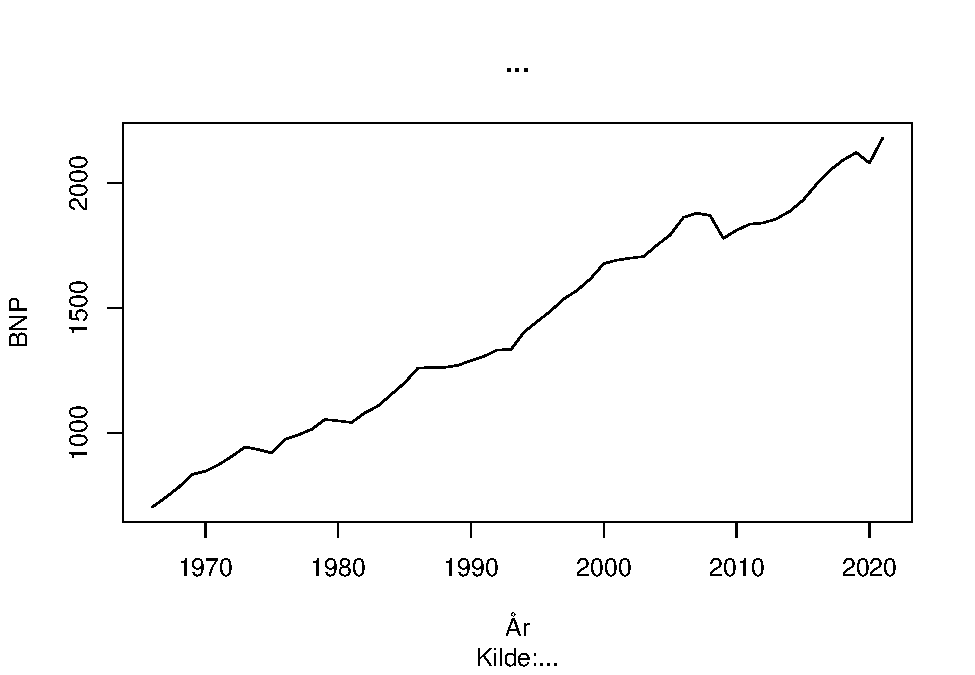
\includegraphics{Rkursus_done_files/figure-latex/unnamed-chunk-3-1.pdf}

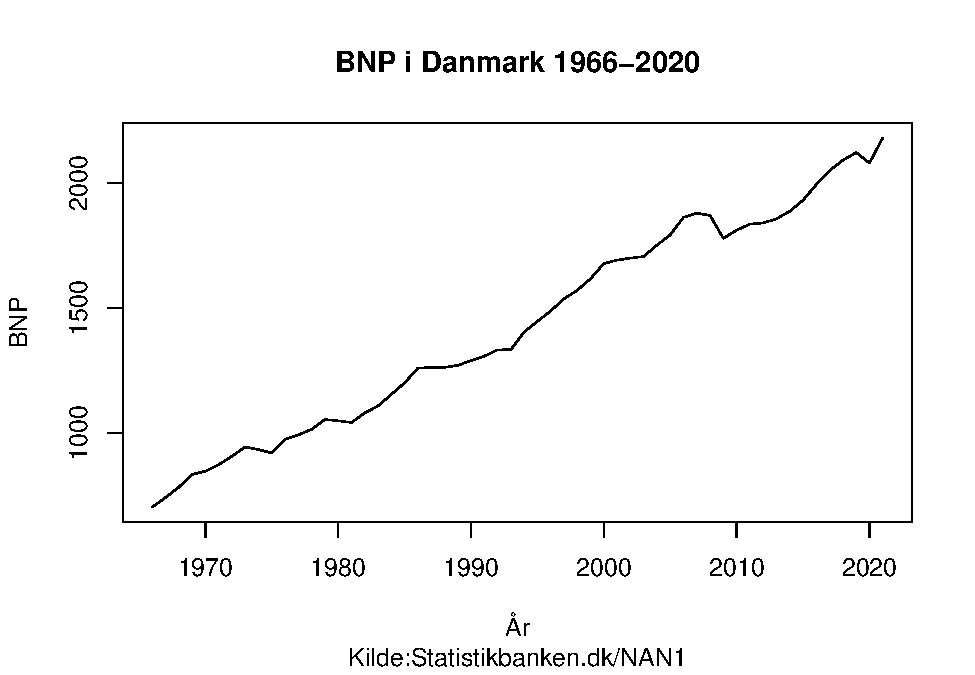
\includegraphics{Rkursus_done_files/figure-latex/unnamed-chunk-4-1.pdf}

\begin{itemize}
\tightlist
\item
  Forklaring:

  \begin{itemize}
  \tightlist
  \item
    `BNP\$Year' angiver `x-variablen'
  \item
    `BNP\$BNP' angiver `y-variablen'
  \item
    `type=``l''\,' angiver linje-type (l=linje, p=punkter, s= steps,
    osv.)
  \item
    `lty=1' angiver linje-type (1=linje, 2=stiplet, 3=prikker, osv.)
  \item
    `lwd' angiver tykkelsen på linjen
  \item
    `xlab="år' angiver titlen på x-aksen
  \item
    `ylab=``BNP''\,' angiver titlen på y-aksen
  \item
    `col=``black''\,' angiver farven (enten ``navn'' eller tal: 1=sort,
    2=rød osv.)
  \item
    `main=``x''\,' angiver en titel på figuren
  \item
    `sub=``y''\,' angiver en bemærkning/kilde, som vises under figuren
  \end{itemize}
\item
  Eksportér figur som PDF/PNG

  \begin{itemize}
  \tightlist
  \item
    Plots \(\rightarrow\) save as image/pdf
  \item
    Indlæs figur i fx Word
  \end{itemize}
\end{itemize}

\hypertarget{uxf8velse-1}{%
\section{Øvelse 1}\label{uxf8velse-1}}

\begin{itemize}
\item
  I denne øvelse, skal I anvende ovenstående `opskrift' til at
  illustrere udviklingen i den danske eksport (data er samme sted som
  BNP)
\item
  Step 1. Importer data
\end{itemize}

\begin{Shaded}
\begin{Highlighting}[]
\NormalTok{Export }\OtherTok{\textless{}{-}} \FunctionTok{read\_excel}\NormalTok{(}\StringTok{"Export.xlsx"}\NormalTok{)}
\FunctionTok{View}\NormalTok{(Export)}
\end{Highlighting}
\end{Shaded}

\begin{itemize}
\tightlist
\item
  Step 2. Observer variable:
\end{itemize}

\begin{Shaded}
\begin{Highlighting}[]
\NormalTok{Export}\SpecialCharTok{$}\NormalTok{Year}
\end{Highlighting}
\end{Shaded}

\begin{verbatim}
##  [1] "1966" "1967" "1968" "1969" "1970" "1971" "1972" "1973" "1974" "1975"
## [11] "1976" "1977" "1978" "1979" "1980" "1981" "1982" "1983" "1984" "1985"
## [21] "1986" "1987" "1988" "1989" "1990" "1991" "1992" "1993" "1994" "1995"
## [31] "1996" "1997" "1998" "1999" "2000" "2001" "2002" "2003" "2004" "2005"
## [41] "2006" "2007" "2008" "2009" "2010" "2011" "2012" "2013" "2014" "2015"
## [51] "2016" "2017" "2018" "2019" "2020" "2021"
\end{verbatim}

\begin{Shaded}
\begin{Highlighting}[]
\NormalTok{Export}\SpecialCharTok{$}\NormalTok{X}
\end{Highlighting}
\end{Shaded}

\begin{verbatim}
##  [1]  123.6  128.2  140.7  149.2  154.9  164.7  173.4  187.8  194.2  192.8
## [11]  199.5  206.6  209.5  232.3  245.3  266.5  275.0  287.6  297.1  315.0
## [21]  319.2  334.7  365.3  382.3  407.3  432.4  433.6  438.9  475.1  488.8
## [31]  511.5  534.5  556.4  619.1  696.9  720.3  751.7  742.7  765.1  824.2
## [41]  909.4  942.6  979.1  888.8  914.9  980.8  992.2 1008.1 1039.7 1076.9
## [51] 1121.2 1175.1 1214.5 1269.3 1189.3 1284.3
\end{verbatim}

\begin{itemize}
\tightlist
\item
  Step 3. vis udviklingen i eksport
\end{itemize}

\begin{Shaded}
\begin{Highlighting}[]
\FunctionTok{plot}\NormalTok{(BNP}\SpecialCharTok{$}\NormalTok{Year,BNP}\SpecialCharTok{$}\NormalTok{BNP,}\AttributeTok{type=}\StringTok{"l"}\NormalTok{,}\AttributeTok{lty=}\DecValTok{1}\NormalTok{,}\AttributeTok{lwd=}\DecValTok{1}\NormalTok{,}\AttributeTok{xlab=}\StringTok{"År"}\NormalTok{,}
\AttributeTok{ylab=}\StringTok{"BNP"}\NormalTok{,}\AttributeTok{col=}\StringTok{"black"}\NormalTok{,}\AttributeTok{main=}\StringTok{"..."}\NormalTok{,}\AttributeTok{sub=}\StringTok{"Kilde:..."}\NormalTok{)}
\end{Highlighting}
\end{Shaded}

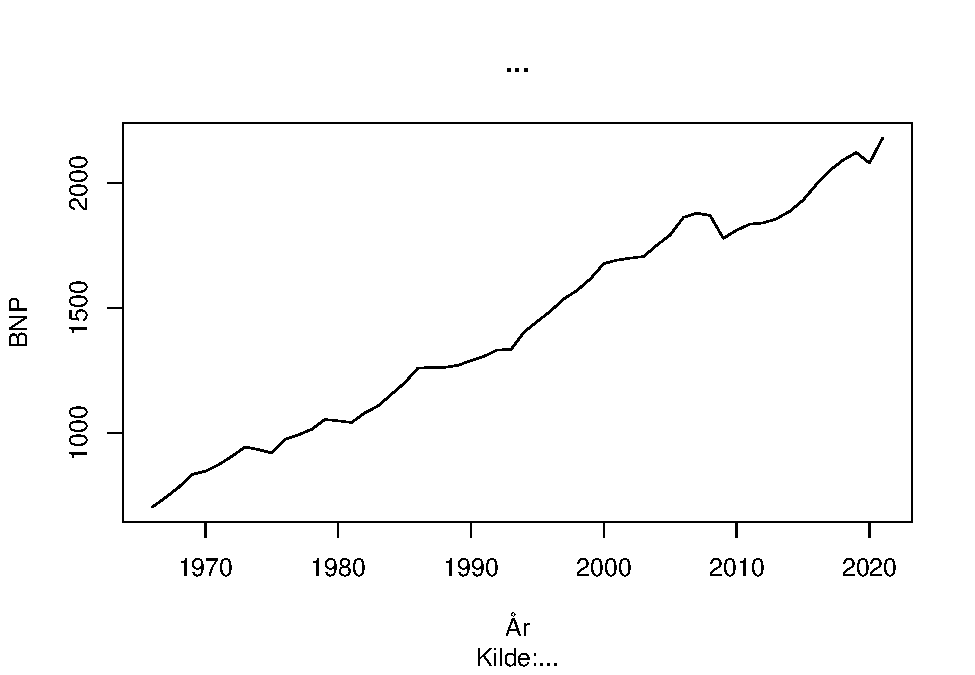
\includegraphics{Rkursus_done_files/figure-latex/unnamed-chunk-7-1.pdf}

\begin{itemize}
\tightlist
\item
  Step 4: Tilføj beskrivelser
\end{itemize}

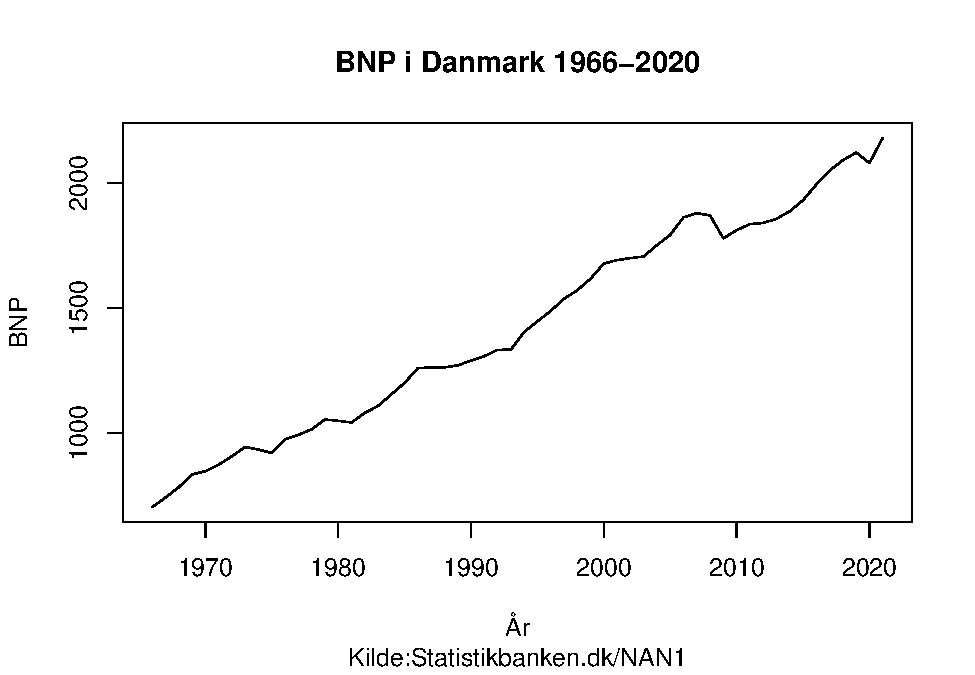
\includegraphics{Rkursus_done_files/figure-latex/unnamed-chunk-8-1.pdf}

\hypertarget{uxf8velse-2}{%
\section{Øvelse 2}\label{uxf8velse-2}}

\begin{itemize}
\tightlist
\item
  I skal nu illustrere udviklingen i såvel eksport som import i samme
  figur

  \begin{itemize}
  \tightlist
  \item
    Hint: I skal tilføje kommandoen lines() efter plot()
  \end{itemize}
\item
  Step 1: Load import data:
\end{itemize}

\begin{Shaded}
\begin{Highlighting}[]
\NormalTok{Import }\OtherTok{\textless{}{-}} \FunctionTok{read\_excel}\NormalTok{(}\StringTok{"Import.xlsx"}\NormalTok{)}
\FunctionTok{View}\NormalTok{(Import)}
\end{Highlighting}
\end{Shaded}

\begin{Shaded}
\begin{Highlighting}[]
\FunctionTok{plot}\NormalTok{(Export}\SpecialCharTok{$}\NormalTok{Year,Export}\SpecialCharTok{$}\NormalTok{X,}\AttributeTok{type=}\StringTok{"l"}\NormalTok{,}\AttributeTok{lty=}\DecValTok{1}\NormalTok{,}\AttributeTok{lwd=}\DecValTok{1}\NormalTok{,}\AttributeTok{xlab=}\StringTok{"År"}\NormalTok{,}
     \AttributeTok{ylab=}\StringTok{"Export/Import"}\NormalTok{,}\AttributeTok{col=}\StringTok{"black"}\NormalTok{,}\AttributeTok{main=}\StringTok{"Import og Eksport"}\NormalTok{,}\AttributeTok{sub=}\StringTok{"Kilde:Statistikbanken"}\NormalTok{);}
\FunctionTok{lines}\NormalTok{(Import}\SpecialCharTok{$}\NormalTok{Year, Import}\SpecialCharTok{$}\NormalTok{Import,}\AttributeTok{type=}\StringTok{"l"}\NormalTok{,}\AttributeTok{lty=}\DecValTok{1}\NormalTok{,}\AttributeTok{lwd=}\DecValTok{1}\NormalTok{,}\AttributeTok{col=}\StringTok{"red"}\NormalTok{)}
\end{Highlighting}
\end{Shaded}

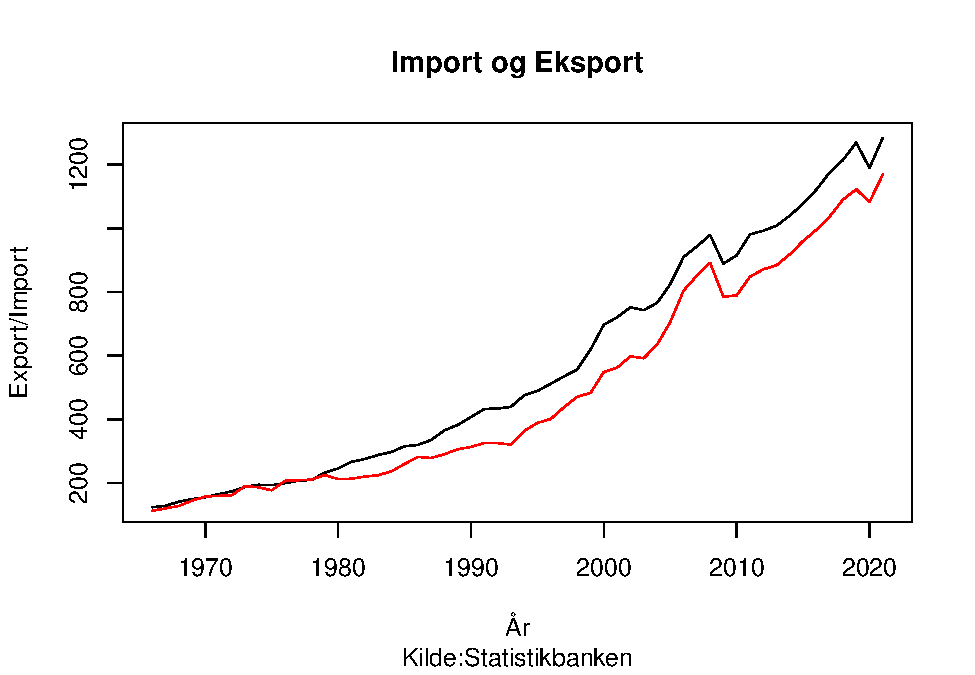
\includegraphics{Rkursus_done_files/figure-latex/unnamed-chunk-10-1.pdf}
- Forklaring: - x angiver variabel 1 (Year) - z angiver variabel 3
(Import)

\begin{itemize}
\tightlist
\item
  Dimensioner på akserne bestemmes af variablen angiver i plot(), men
  kan styres manuelt ved at tilføje kommandoen ylim=c(x1,y1) i plot()
\end{itemize}

\begin{Shaded}
\begin{Highlighting}[]
\FunctionTok{plot}\NormalTok{(Export}\SpecialCharTok{$}\NormalTok{Year,Export}\SpecialCharTok{$}\NormalTok{X,}\AttributeTok{type=}\StringTok{"l"}\NormalTok{,}\AttributeTok{lty=}\DecValTok{1}\NormalTok{,}\AttributeTok{lwd=}\DecValTok{1}\NormalTok{,}\AttributeTok{xlab=}\StringTok{"År"}\NormalTok{,}
\AttributeTok{ylab=}\StringTok{"BNP"}\NormalTok{,}\AttributeTok{col=}\StringTok{"black"}\NormalTok{,}\AttributeTok{main=}\StringTok{"Import og Eksport"}\NormalTok{,}\AttributeTok{sub=}\StringTok{"Kilde:Statistikbanken"}\NormalTok{,}\AttributeTok{ylim=}\FunctionTok{c}\NormalTok{(}\DecValTok{100}\NormalTok{,}\DecValTok{1300}\NormalTok{));}
\FunctionTok{lines}\NormalTok{(Import}\SpecialCharTok{$}\NormalTok{Year,Import}\SpecialCharTok{$}\NormalTok{Import,}\AttributeTok{type=}\StringTok{"l"}\NormalTok{,}\AttributeTok{lty=}\DecValTok{1}\NormalTok{,}\AttributeTok{lwd=}\DecValTok{1}\NormalTok{,}\AttributeTok{col=}\StringTok{"red"}\NormalTok{);}\FunctionTok{grid}\NormalTok{()}
\end{Highlighting}
\end{Shaded}

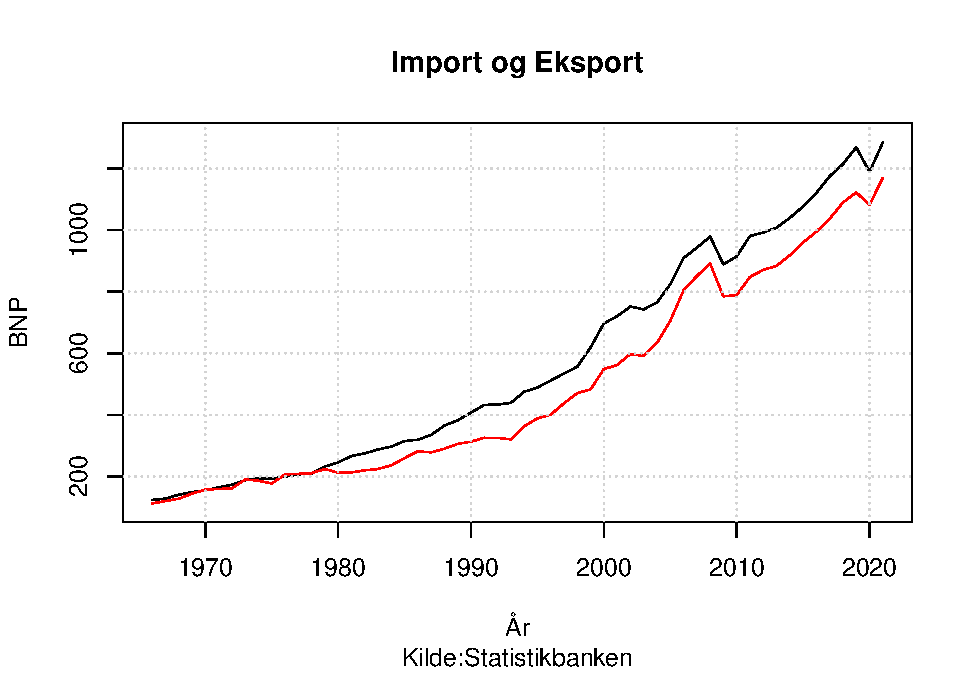
\includegraphics{Rkursus_done_files/figure-latex/unnamed-chunk-11-1.pdf}
- x1 angiver her den nedre værdi på aksen, mens y1 angiver øvre værdi på
aksen - Når man har to linjer bør man tilføje en legend, for at øge
læsevenligheden af figuren: - Hint: tilføj kommandoen

\begin{Shaded}
\begin{Highlighting}[]
\FunctionTok{plot}\NormalTok{(Export}\SpecialCharTok{$}\NormalTok{Year,Export}\SpecialCharTok{$}\NormalTok{X,}\AttributeTok{type=}\StringTok{"l"}\NormalTok{,}\AttributeTok{lty=}\DecValTok{1}\NormalTok{,}\AttributeTok{lwd=}\DecValTok{1}\NormalTok{,}\AttributeTok{xlab=}\StringTok{"År"}\NormalTok{,}
\AttributeTok{ylab=}\StringTok{"BNP"}\NormalTok{,}\AttributeTok{col=}\StringTok{"black"}\NormalTok{,}\AttributeTok{main=}\StringTok{"Import og Eksport"}\NormalTok{,}\AttributeTok{sub=}\StringTok{"Kilde:Statistikbanken"}\NormalTok{,}\AttributeTok{ylim=}\FunctionTok{c}\NormalTok{(}\DecValTok{100}\NormalTok{,}\DecValTok{1300}\NormalTok{));}
\FunctionTok{lines}\NormalTok{(Import}\SpecialCharTok{$}\NormalTok{Year,Import}\SpecialCharTok{$}\NormalTok{Import,}\AttributeTok{type=}\StringTok{"l"}\NormalTok{,}\AttributeTok{lty=}\DecValTok{1}\NormalTok{,}\AttributeTok{lwd=}\DecValTok{1}\NormalTok{,}\AttributeTok{col=}\StringTok{"red"}\NormalTok{); }
\FunctionTok{legend}\NormalTok{(}\AttributeTok{x=}\DecValTok{1970}\NormalTok{,}\AttributeTok{y=} \DecValTok{1200}\NormalTok{,}\AttributeTok{legend=}\FunctionTok{c}\NormalTok{(}\StringTok{"Export"}\NormalTok{,}\StringTok{"Import"}\NormalTok{),}\AttributeTok{lty=}\DecValTok{1}\NormalTok{,}\AttributeTok{lwd=}\DecValTok{2}\NormalTok{,}
       \AttributeTok{col=}\FunctionTok{c}\NormalTok{(}\StringTok{"Black"}\NormalTok{,}\StringTok{"Red"}\NormalTok{),}\AttributeTok{bty=}\StringTok{"n"}\NormalTok{); }\FunctionTok{grid}\NormalTok{()}
\end{Highlighting}
\end{Shaded}

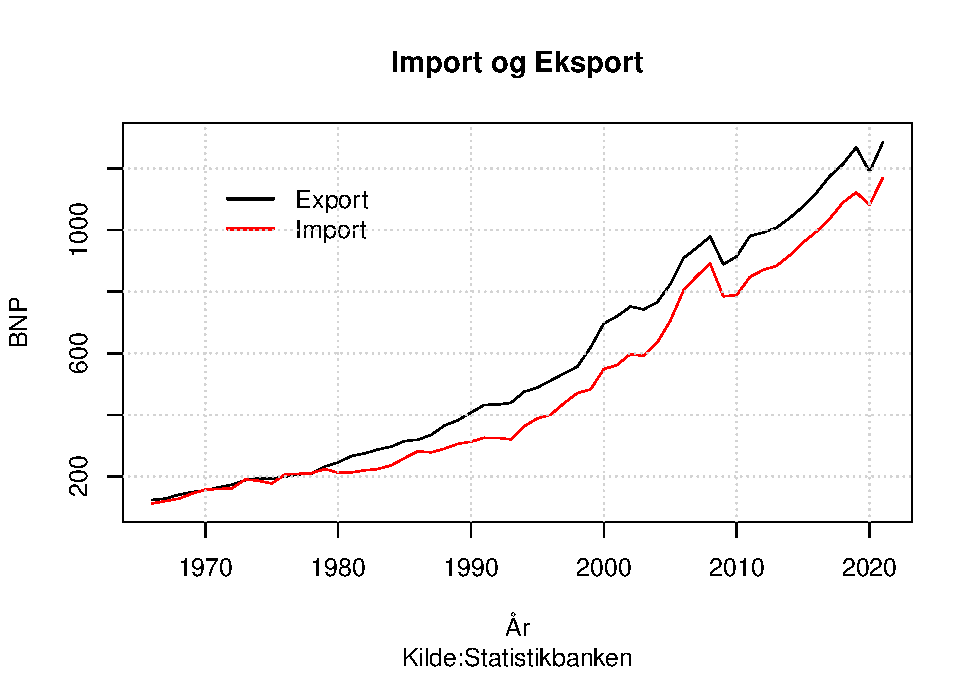
\includegraphics{Rkursus_done_files/figure-latex/unnamed-chunk-12-1.pdf}
- Forklaring: - x = placering på x-aksen - y = placering på y-aksen -
var1 = navn på variabel 1 - var2 = navn på variable 2 - lty = linje-type
- lwd = linje-tykkelse - cvar1 = farve på linje for variable 1 - cvar2 =
farve på linje for variable 2 - bty=``n'' - ønskes ramme omkring legend,
slettes dette led.

\hypertarget{uxf8velse}{%
\section{Øvelse}\label{uxf8velse}}

\begin{itemize}
\tightlist
\item
  I skal nu illustrere udviklingen i såvel investeringer som BNP i samme
  figur

  \begin{itemize}
  \tightlist
  \item
    Hint: Størrelsesforholdet mellem de to variable taler for at plotte
    et diagram med to y-akser
  \end{itemize}
\item
  Step 1: Importer data
\end{itemize}

\begin{Shaded}
\begin{Highlighting}[]
\NormalTok{Inv }\OtherTok{\textless{}{-}} \FunctionTok{read\_excel}\NormalTok{(}\StringTok{"Inv.xlsx"}\NormalTok{)}
\end{Highlighting}
\end{Shaded}

\begin{Shaded}
\begin{Highlighting}[]
\FunctionTok{plot}\NormalTok{(BNP}\SpecialCharTok{$}\NormalTok{Year,BNP}\SpecialCharTok{$}\NormalTok{BNP, }\AttributeTok{ylim=}\FunctionTok{c}\NormalTok{(}\DecValTok{600}\NormalTok{,}\DecValTok{2300}\NormalTok{), }\AttributeTok{xlab=}\StringTok{"Year"}\NormalTok{, }\AttributeTok{ylab=}\StringTok{"BNP"}\NormalTok{, }
\AttributeTok{type=}\StringTok{"l"}\NormalTok{,}\AttributeTok{col=}\StringTok{"black"}\NormalTok{, }\AttributeTok{main=}\StringTok{"BNP og Investeringer"}\NormalTok{);}\FunctionTok{axis}\NormalTok{(}\DecValTok{2}\NormalTok{, }\AttributeTok{ylim=}\FunctionTok{c}\NormalTok{(}\DecValTok{600}\NormalTok{,}\DecValTok{2300}\NormalTok{),}\AttributeTok{col=}\StringTok{"black"}\NormalTok{) }
  
\FunctionTok{par}\NormalTok{(}\AttributeTok{new=}\ConstantTok{TRUE}\NormalTok{)}
  
\FunctionTok{plot}\NormalTok{(Inv}\SpecialCharTok{$}\NormalTok{Year,Inv}\SpecialCharTok{$}\NormalTok{I, }\AttributeTok{ylab=} \StringTok{""}\NormalTok{, }\AttributeTok{xlab =} \StringTok{""}\NormalTok{, }\AttributeTok{ylim=}\FunctionTok{c}\NormalTok{(}\DecValTok{100}\NormalTok{,}\DecValTok{600}\NormalTok{), }
    \AttributeTok{axes=}\ConstantTok{FALSE}\NormalTok{, }\AttributeTok{type=}\StringTok{"l"}\NormalTok{, }\AttributeTok{col=}\StringTok{"red"}\NormalTok{);}\FunctionTok{axis}\NormalTok{(}\DecValTok{4}\NormalTok{, }\AttributeTok{ylim=}\FunctionTok{c}\NormalTok{(}\DecValTok{100}\NormalTok{,}\DecValTok{600}\NormalTok{), }\AttributeTok{col=}\StringTok{"red"}\NormalTok{,}\AttributeTok{col.axis=}\StringTok{"red"}\NormalTok{)}
\end{Highlighting}
\end{Shaded}

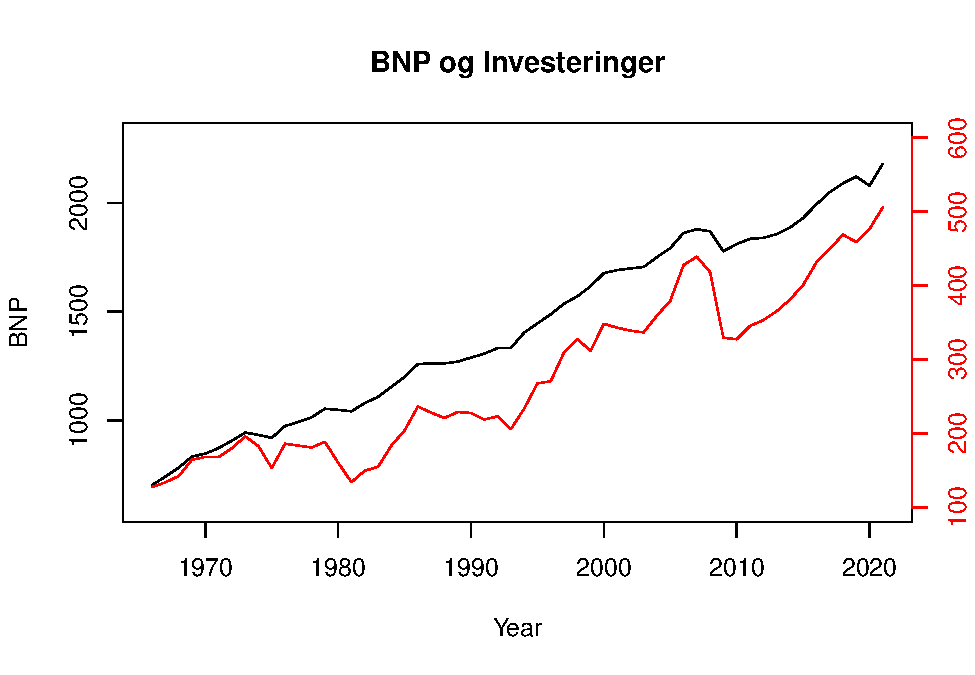
\includegraphics{Rkursus_done_files/figure-latex/unnamed-chunk-14-1.pdf}
Forklaring: - x = variabel 1 - y = variabel 2 - x1 = nedre værdi y-akse
1 - y1 = øvre værdi y-akse 1 - x = variabel 1 - z = variabel 3 - x2 =
nedre værdi y-akse 2 - y2 = øvre værdi y-akse 2

\hypertarget{uxf8velse-3}{%
\section{Øvelse}\label{uxf8velse-3}}

Undersøg grafisk nedenstående to påstande om den danske økonomi:

\begin{enumerate}
\def\labelenumi{\arabic{enumi}.}
\tightlist
\item
  Realvæksten i den årlige BNP var ikke negativ i perioden 1982-2007
\end{enumerate}

\begin{Shaded}
\begin{Highlighting}[]
\FunctionTok{plot}\NormalTok{(BNP}\SpecialCharTok{$}\NormalTok{Year,BNP}\SpecialCharTok{$}\NormalTok{BNP, }\AttributeTok{xlim =} \FunctionTok{c}\NormalTok{(}\DecValTok{1982}\NormalTok{,}\DecValTok{2007}\NormalTok{), }\AttributeTok{xlab=}\StringTok{"Year"}\NormalTok{, }\AttributeTok{ylab=}\StringTok{"BNP"}\NormalTok{, }
\AttributeTok{type=}\StringTok{"l"}\NormalTok{,}\AttributeTok{col=}\StringTok{"black"}\NormalTok{, }\AttributeTok{main=}\StringTok{"BNP"}\NormalTok{);}\FunctionTok{axis}\NormalTok{(}\DecValTok{2}\NormalTok{, }\AttributeTok{ylim=}\FunctionTok{c}\NormalTok{(}\DecValTok{600}\NormalTok{,}\DecValTok{2300}\NormalTok{),}\AttributeTok{col=}\StringTok{"black"}\NormalTok{)}
\end{Highlighting}
\end{Shaded}

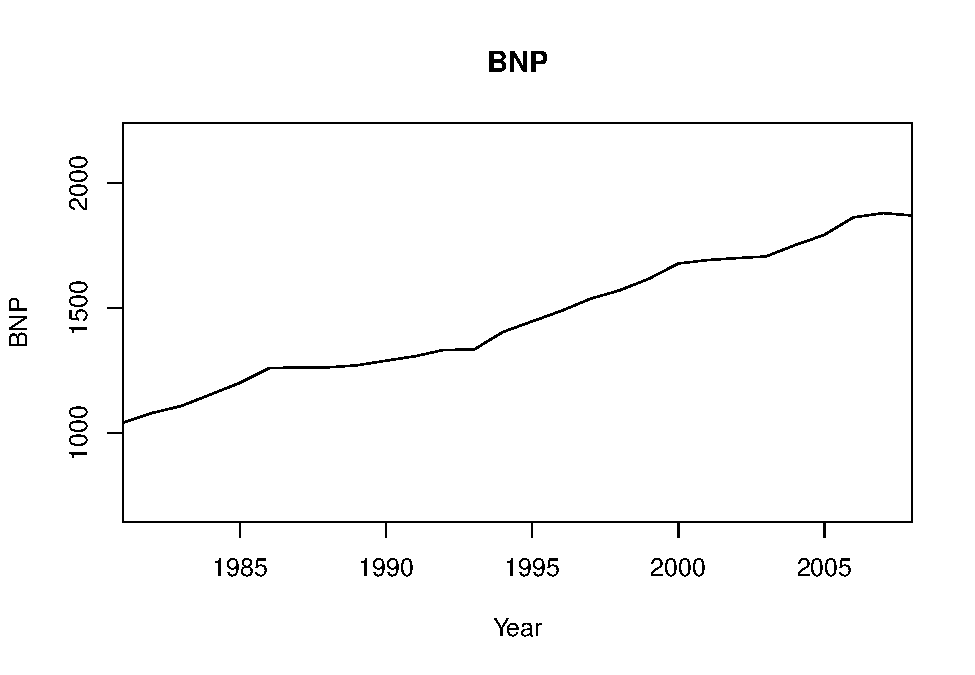
\includegraphics{Rkursus_done_files/figure-latex/unnamed-chunk-15-1.pdf}

\begin{Shaded}
\begin{Highlighting}[]
\FunctionTok{plot}\NormalTok{(BNP}\SpecialCharTok{$}\NormalTok{Year[}\SpecialCharTok{{-}}\DecValTok{1}\NormalTok{],}\FunctionTok{diff}\NormalTok{(BNP}\SpecialCharTok{$}\NormalTok{BNP), }\AttributeTok{xlim =} \FunctionTok{c}\NormalTok{(}\DecValTok{1982}\NormalTok{,}\DecValTok{2007}\NormalTok{), }\AttributeTok{xlab=}\StringTok{"Year"}\NormalTok{, }\AttributeTok{ylab=}\StringTok{"BNP"}\NormalTok{, }
\AttributeTok{type=}\StringTok{"l"}\NormalTok{,}\AttributeTok{col=}\StringTok{"black"}\NormalTok{, }\AttributeTok{main=}\StringTok{"Ændring i BNP"}\NormalTok{);}\FunctionTok{axis}\NormalTok{(}\DecValTok{2}\NormalTok{, }\AttributeTok{ylim=}\FunctionTok{c}\NormalTok{(}\DecValTok{600}\NormalTok{,}\DecValTok{2300}\NormalTok{),}\AttributeTok{col=}\StringTok{"black"}\NormalTok{) }
\end{Highlighting}
\end{Shaded}

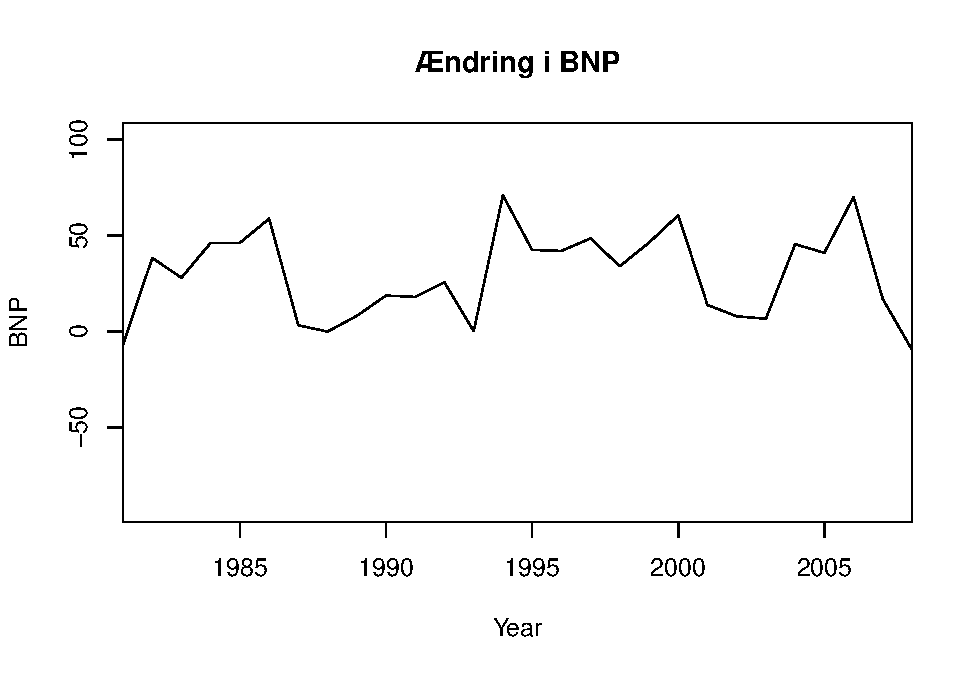
\includegraphics{Rkursus_done_files/figure-latex/unnamed-chunk-16-1.pdf}

\begin{enumerate}
\def\labelenumi{\arabic{enumi}.}
\setcounter{enumi}{1}
\tightlist
\item
  Trods effekterne fra Corona, var beskæftigelsen højere i 2020 end i
  2018
\end{enumerate}

Indlæser først data for employment:

\begin{Shaded}
\begin{Highlighting}[]
\NormalTok{Employment }\OtherTok{\textless{}{-}} \FunctionTok{read\_excel}\NormalTok{(}\StringTok{"Employment.xlsx"}\NormalTok{)}
\end{Highlighting}
\end{Shaded}

Vi kan måske se det med et plot?

\begin{Shaded}
\begin{Highlighting}[]
\FunctionTok{plot}\NormalTok{(Employment}\SpecialCharTok{$}\NormalTok{Year,Employment}\SpecialCharTok{$}\NormalTok{Emp, }\AttributeTok{xlab=}\StringTok{"Year"}\NormalTok{, }\AttributeTok{ylab=}\StringTok{"EMP"}\NormalTok{, }
\AttributeTok{type=}\StringTok{"l"}\NormalTok{,}\AttributeTok{col=}\StringTok{"black"}\NormalTok{, }\AttributeTok{main=}\StringTok{"Beskæftigelse"}\NormalTok{); }\FunctionTok{grid}\NormalTok{()}
\end{Highlighting}
\end{Shaded}

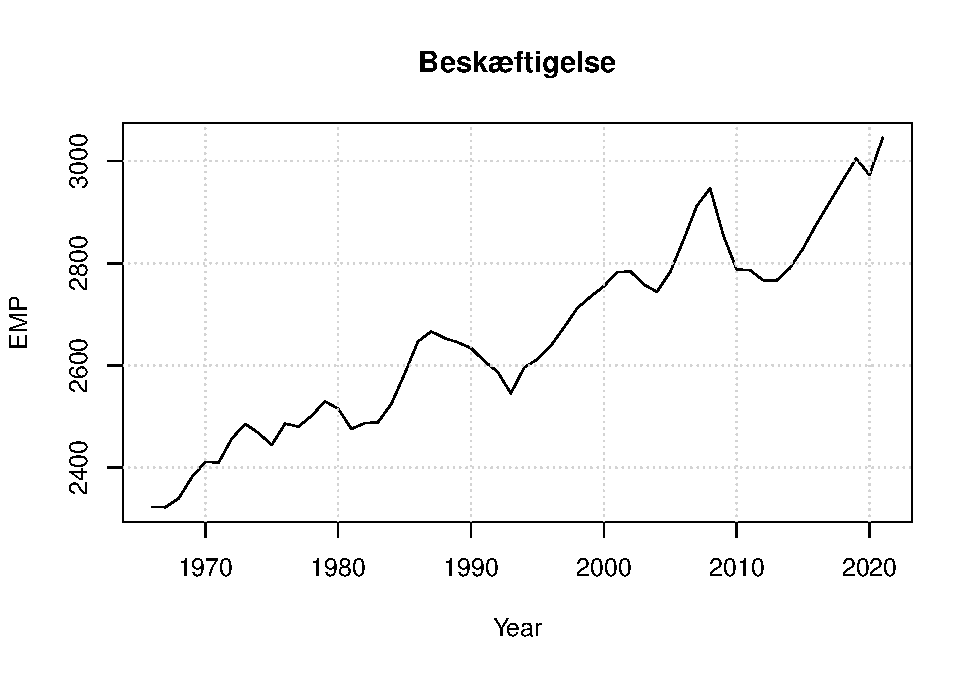
\includegraphics{Rkursus_done_files/figure-latex/unnamed-chunk-18-1.pdf}

Hvis det er svært at se kan vi også bare kigge direkte i variablen

\begin{Shaded}
\begin{Highlighting}[]
\FunctionTok{View}\NormalTok{(Employment)}
\end{Highlighting}
\end{Shaded}

Vi kan se 2018 har observation 53 og 2020 observation 55 Dermed kan vi
sammenligne disse

\begin{Shaded}
\begin{Highlighting}[]
\NormalTok{Emp\_2018}\OtherTok{=}\NormalTok{ Employment}\SpecialCharTok{$}\NormalTok{Emp[}\DecValTok{53}\NormalTok{]}
\NormalTok{Emp\_2020}\OtherTok{=}\NormalTok{ Employment}\SpecialCharTok{$}\NormalTok{Emp[}\DecValTok{55}\NormalTok{]}
\end{Highlighting}
\end{Shaded}

Vi kan faktisk direkte spørge R hvilken der er størst

\begin{Shaded}
\begin{Highlighting}[]
\NormalTok{Emp\_2018 }\SpecialCharTok{\textgreater{}}\NormalTok{ Emp\_2020}
\end{Highlighting}
\end{Shaded}

\begin{verbatim}
## [1] FALSE
\end{verbatim}

\begin{Shaded}
\begin{Highlighting}[]
\NormalTok{Emp\_2020 }\SpecialCharTok{\textgreater{}}\NormalTok{ Emp\_2018}
\end{Highlighting}
\end{Shaded}

\begin{verbatim}
## [1] TRUE
\end{verbatim}

Vi kan se at employment i 2020 var større end i 2018

  \bibliography{Bibliography.bib}

\end{document}
